\chapter{Physical Setup}\label{ch:physsetup}

This chapter explains how the setup is built.
Going into detail about the pump type used,
centrifugal pumps, since they determine the major dynamics of the system.
The other components, pipes, valves and sensors are also explained,
but in less detail.

To give a general overview of the setup,
Figure \ref{fig:setup_photo} shows the front view of the setup,
with all three pumps (red and black) and their individual sensors (blue) visible.
Also visible are the control valve, the target computer,
parts of the electrical wiring and parts of the piping.

\begin{figure}[h]
    \centering
    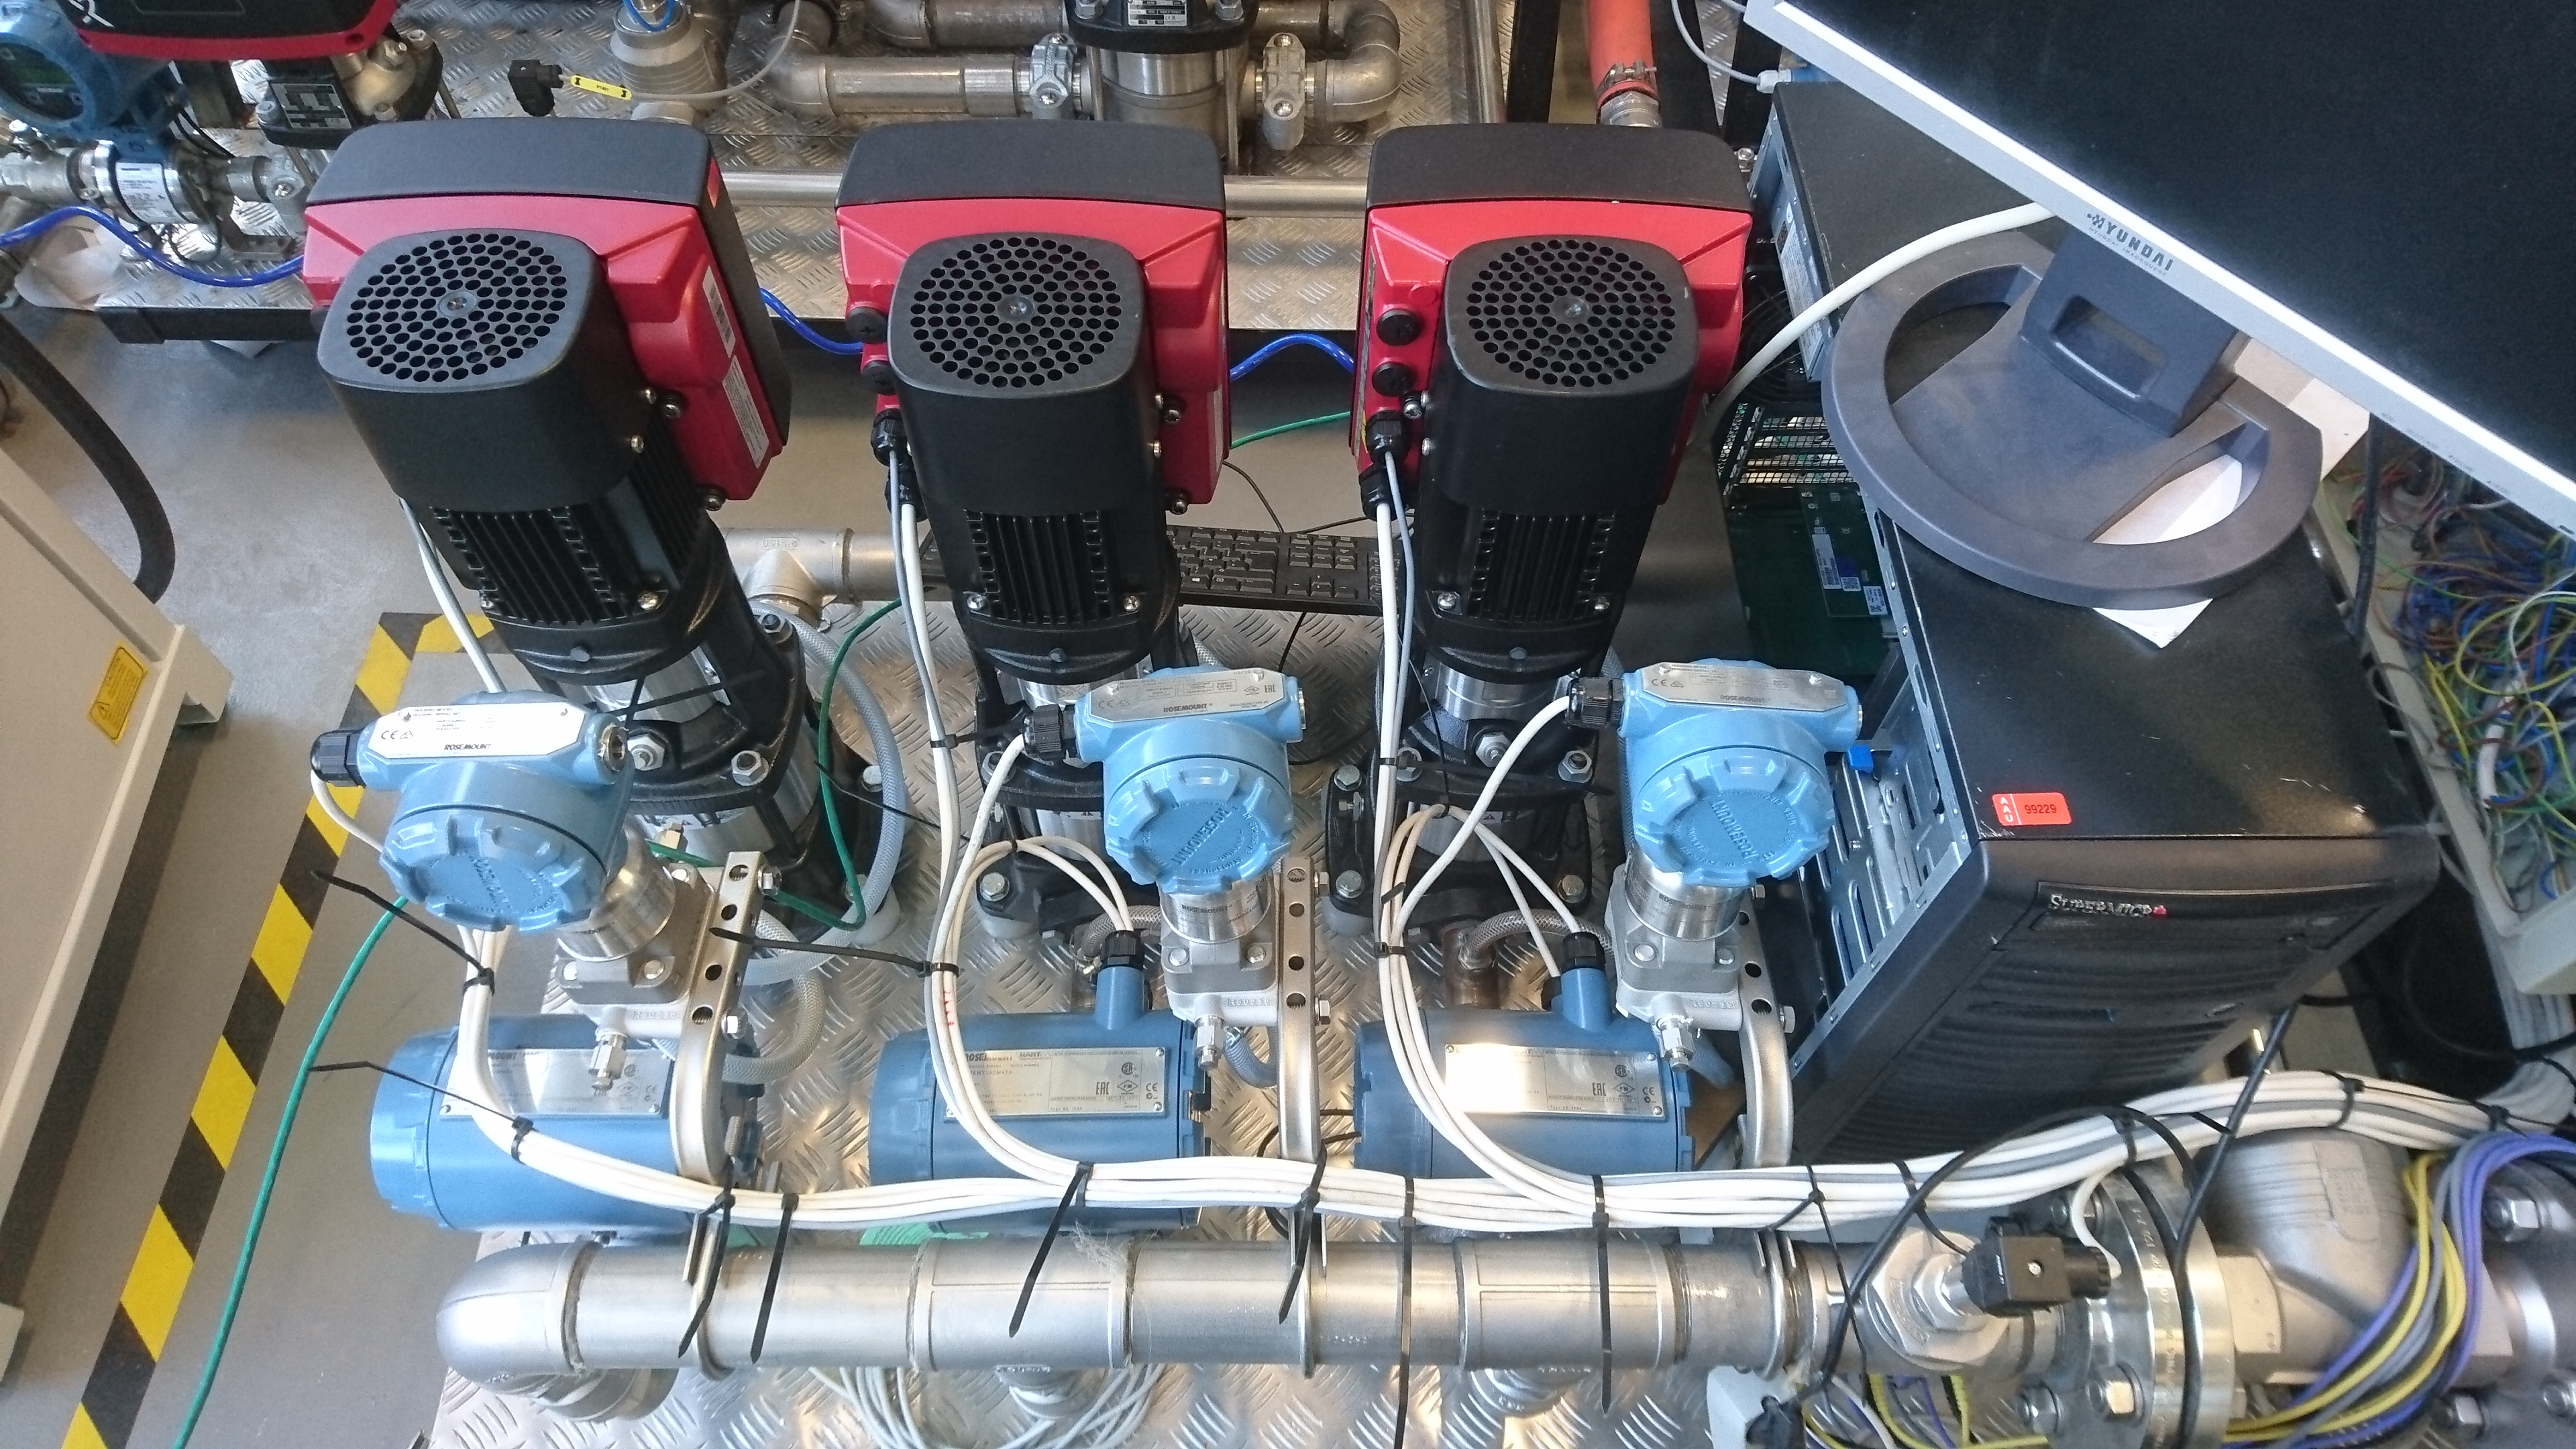
\includegraphics[width=0.8\textwidth]{photos/setup_photo}
    \caption{Photo of the setup}
    \label{fig:setup_photo}
\end{figure}

Not visible on this photo are the power sensor and the water tank.

A schematic overview of the system is available in Appendix \ref{app:overview}.

This setup was already available for use with student projects
and two other groups used it simultaneously,
which is why no alterations were taken.

\section{Centrifugal Pumps}
A pump is a device used to move liquid through a piping system and to 
raise the pressure of the liquid.
The rise in pressure is often necessary for processes upstream
or to overcome a rise in the pipeline.
We will focus on explaining and describing only centrifugal pumps,
since this is the type of pump present in our setup. 

\subsection{Principle}
In 1689, physicist Denis Papin invented the centrifugal pump. 
It is the most commonly used type of pump, due to its simple construction,
relative low cost, reliability and quiet operation.

The pump is built on a simple principle: Liquid is led to the impeller hub
and by means of the centrifugal force it is flung towards the periphery of 
the impeller. 

Figure \ref{fig:pump_sections} shows two cross sections of a centrifugal pump,
showing the flow of liquid through the pump.
\begin{figure}[h]
    \centering
    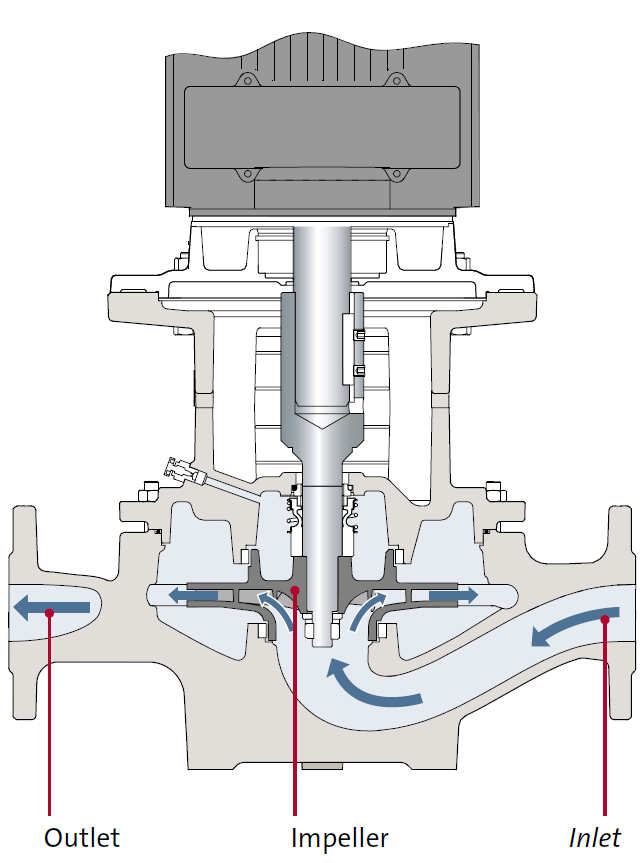
\includegraphics[width=0.3\linewidth]{figures/pump_cross_section.PNG}
    \qquad
    \hspace{0.1\textwidth}
    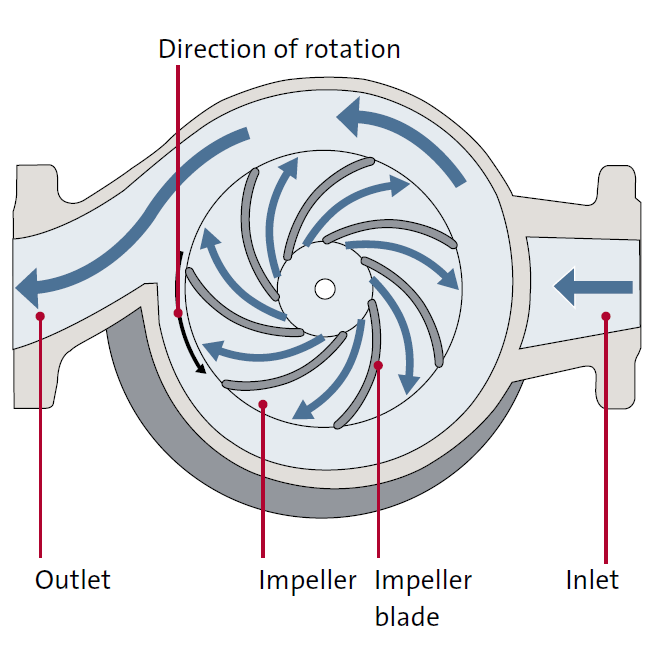
\includegraphics[width=0.3\linewidth]{figures/pump_above_view.PNG}
    \caption{Centrifugal Pump}
    \label{fig:pump_sections}
\end{figure}
\newpage

The fluid is sucked into the impeller at the impeller eye and flows through
the impeller channels formed by the blades between the shroud and hub.
The blades of the rotating impeller transfer energy to the fluid by
increasing velocity and pressure.

The design of the impeller depends on the requirements for application,
pressure and flow. The impeller is the primary component determining the pump performance. 
Pumps variants are often created only by modifying the impeller.

Changing the impeller size of a pump does not influence all output characteristics equally,
but the change can be modelled with the Affinity Laws.

\subsection{Affinity Laws}\label{sub:afflaws}
Affinity laws are mathematical relationships that provide a way to estimate the 
changes in performance of a pump, as a result of a change in one of the basic pump variables.
In it's simplest form, the term law, means a principle that has been proven true for all cases.
\todo[color=03physicalSetup]{Still not sure about that sentence with all cases...}

Equations \ref{eq:afflaw1} show the relations between a change in motor speeds $N$
to flow $Q$, head $H$ and power $P$.

\begin{equation}
	\frac{Q_1}{Q_2} = \left(\frac{N_1}{N_2}\right)
	\hspace{10mm}
	\frac{H_1}{H_2} = \left(\frac{N_1}{N_2}\right)^2
	\hspace{10mm}
	\frac{P_1}{P_2} = \left(\frac{N_1}{N_2}\right)^3
	\label{eq:afflaw1}	
\end{equation}
\cite{Volk2014}\\\\
Similarly, the equations \ref{eq:afflaw2} show the relation between a change in impeller diameter $D$
to  $Q$, $H$ and $P$.

\begin{equation}
	\frac{Q_1}{Q_2} = \left(\frac{D_1}{D_2}\right)
	\hspace{10mm}
	\frac{H_1}{H_2} = \left(\frac{D_1}{D_2}\right)^2
	\hspace{10mm}
	\frac{P_1}{P_2} = \left(\frac{D_1}{D_2}\right)^3
	\label{eq:afflaw2}	
\end{equation}
\cite{Volk2014}

\subsection{Performance Curves}
Performance curves are a very widespread way to compare pumps
and estimate what pump is needed in a specific application.
We included them in this report,
because they also help understanding the relations of $Q$, $H$ and $\omega P$/$N$.

\subsubsection{Pump Head Curve}
A QH-curve or pump curve defines the head as a function of the flow. 
The flow is the rate of the fluid going through the pump.
It is generally stated in cubic meters per hour ($\frac{m^{3}}{h}$).
Figure \ref{fig:typicalPumpCurve} shows a typical pump head curve.
Interesting to notice is,
that the pressure decreases quadratically with the flow.
This can be explained with the Affinity laws mentioned earlier.

\begin{figure}[h]
	\centering
	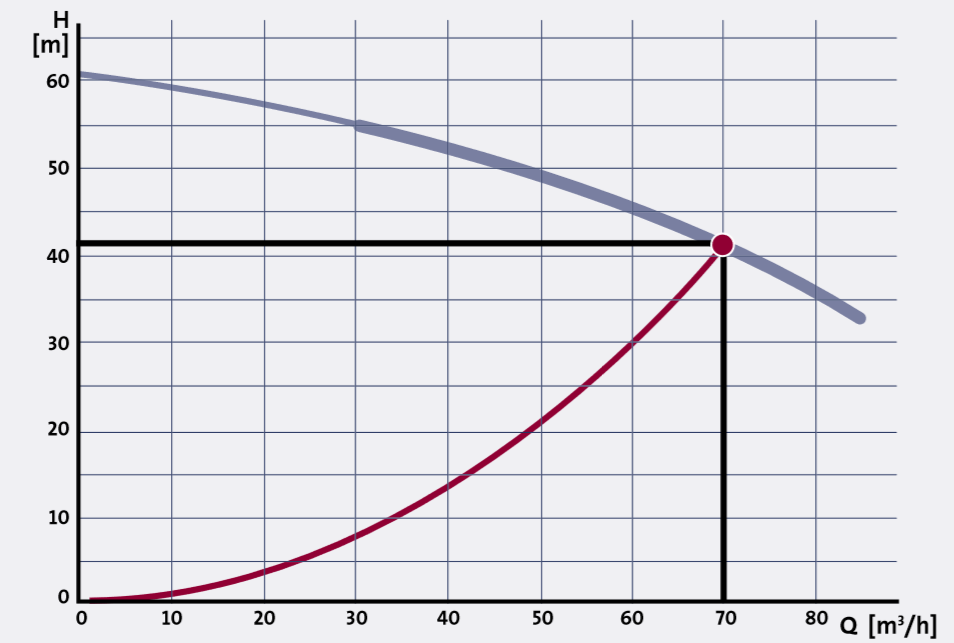
\includegraphics[width=0.8\textwidth]{figures/03physicalSetup/typicalHeadCurve.PNG}
	\caption{Typical Pump Head Curve}
	\label{fig:typicalPumpCurve}
\end{figure}

\subsubsection{Power Consumption Curve}
The power consumption $P_{el}$ is another key factor,
when choosing a pump for an application.
The typical between $Q$ and $P_{el}$ can be seen in Figure \ref{fig:typicalPowerConsumptionCurve}.
Generally, the power consumption increases with the flow.

\begin{figure}[h]
	\centering
	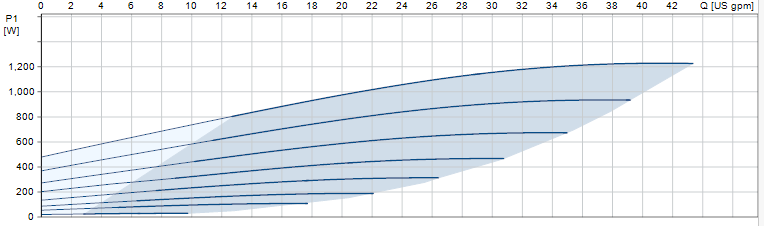
\includegraphics[width=0.9\textwidth]{figures/03physicalSetup/typicalPowerConsumptionCurve.PNG}
	\caption{Typical Power Consumption Curve}
	\label{fig:typicalPowerConsumptionCurve}
\end{figure}

\subsubsection{Efficiency Curve}
The efficiency $\eta$ of a pump is the relation between the power delivered from the pump to the water $P_{hyd}$ and $P_{el}$.
Figure \ref{fig:typicalEfficiencyCurve} shows 
a typical efficiency curve of a pump.

\begin{figure}[h]
	\centering
	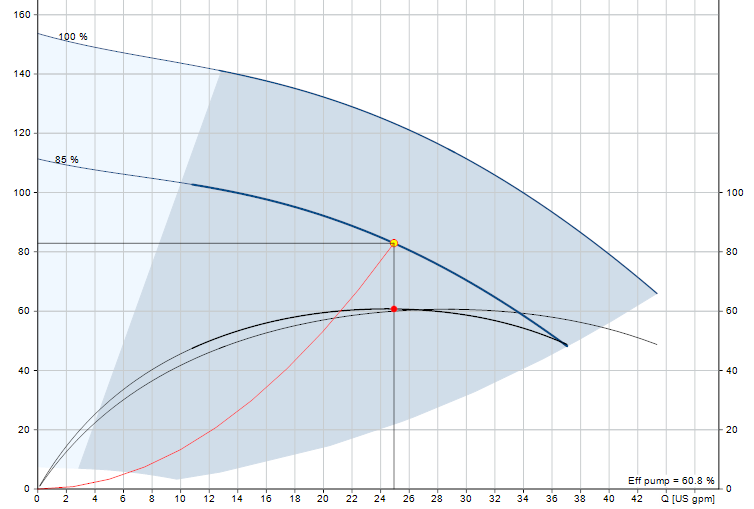
\includegraphics[width=0.9\textwidth]{figures/03physicalSetup/typicalEfficiencyCurve.PNG}
	\caption{Typical Efficiency Curve}
	\label{fig:typicalEfficiencyCurve}
\end{figure}
Noticeable here is,
that $\eta$ does not linearly correlate to $P_{el}$.

\subsubsection{NPSH - Curve (Net Positive Suction Head)}
The Net Positive Suction head (NPSH) is the minimum required pressure that has to be present at the inlet to avoid cavitation.
The NPSH increases with the flow.
Figure \ref{fig:typicalNPSHCurve} shows a typical NPSH - Curve.

\begin{figure}[h]
	\centering
	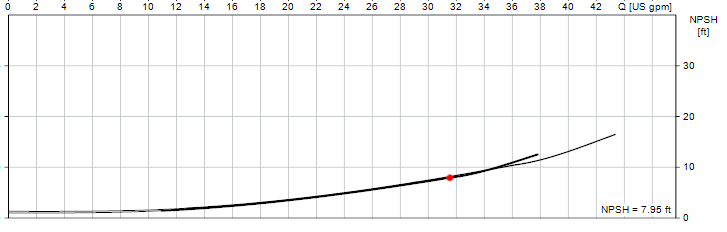
\includegraphics[width=0.9\textwidth]{figures/03physicalSetup/typicalNPSHCurve.PNG}
	\caption{Typical NPSH Curve}
	\label{fig:typicalNPSHCurve}
\end{figure}

\section{Pipes}
Pipes are a way of transporting liquids or gasses, inside a controllable environment.
They are used to interconnect the pumps and the tank and other peripherals.
One common analogy compares them to wires in electrical circuits.

Based on their diameters, material and shape,
they introduce resistance to the flow of the pumped medium.
Staying with the analogy to electrical circuits,
this can be compared to the cross sectional area and the specific resistance of a wire material.

\section{Valves}
A valve is a device used to regulate the flow of a gas or liquid through a piping system.
Valves can be actuated by different means, such as air pressure, electric motors or rotary handles.
The valve present in our setup is a Beukert valve. \todo[color=03physicalSetup]{look up the actual name of the valve}
In our project, we are not using the valve for regulatory purposes,
but only to simulate disturbances in the system.


\section{Target PC}
A target PC is often used when a setup has to be run in real-time.
In our setup it is a desktop PC running xPC target,
a real-time capable OS.
It is equipped with a PCI card to collect the data from all sensors.
In other cases a different PC setup might be used,
with application specific hardware.
Because the target PC is not a key part of this project,
but merely a tool,
we will not go into detail about it.
\todo[color=03physicalSetup]{find some source (speedgoat?)}

\section{Sensors}
When we started the project,
the setup was already equipped with several sensors.
This section will briefly explain what sensors are used.

\subsection*{Flow Meter}
Downstream from  each pump, a magnetic flow meter (MFM) is installed to measure the flow.
\todo[color=03physicalSetup]{look up the sensor}
Their digital gauge was used to calibrate the sensors data output to cubic meters per hour ($\frac{m^3}{h}$).

\subsection*{Power Sensor}
A power sensor was used to closely monitor the power delivered to the pumps.
This power works like a digital multimeter,
measuring voltage $U$ and current $I$.
From those measurements it calculates the power $P$.
\todo[color=03physicalSetup]{look up the sensor}
This sensor has a digital display, where $U$ [$V$], $I$ [$A$] and $P$ [$kW$] are displayed,
which we used to calibrate the output to $kW$.

\subsection*{$\Delta$Pressure Sensor}
Pressure sensors are installed across each pump,
measuring the pressure difference between the inlet and the outlet of the pump.
\todo[color=03physicalSetup]{look up the sensor}
Because they didn't have a visual representation of their measurements
and all our previous calculations of sensor calibration fit with previous work done on the setup
\todo[color=03physicalSetup]{cite Kaspers work},
we chose to rely on previous calibration and inherited their conversion.
After this conversion they output data is measured in $bar$.